\chapter{Bedienungsanleitung}\label{chap:bedienungsanleitung}

Im Normalfall liegt der Visual-Megesort als Datei mit der Endung \texttt{.jar} vor. Die Dateiendung JAR kennzeichnet Archive, die mehrere Java-Dateien und deren Metainformationen enthalten. Um die Datei ausführen zu können, muss die \texttt{Java Runtime Environment} installiert sein. Die Laufzeitumgebung kann gegebenenfalls kostenlos im Internet heruntergeladen werden.

Die Anwendung kann man durch einen Doppelklick, oder aus der Konsole durch den folgenden Aufruf starten.

\begin{verbatim}
java -jar Visual-Mergesort.jar
\end{verbatim}

Startet man die Applikation, so öffnet sich folgendes Fenster (Abbildung \ref{figure:start-app})

\begin{figure}[!htb]
    \centering
      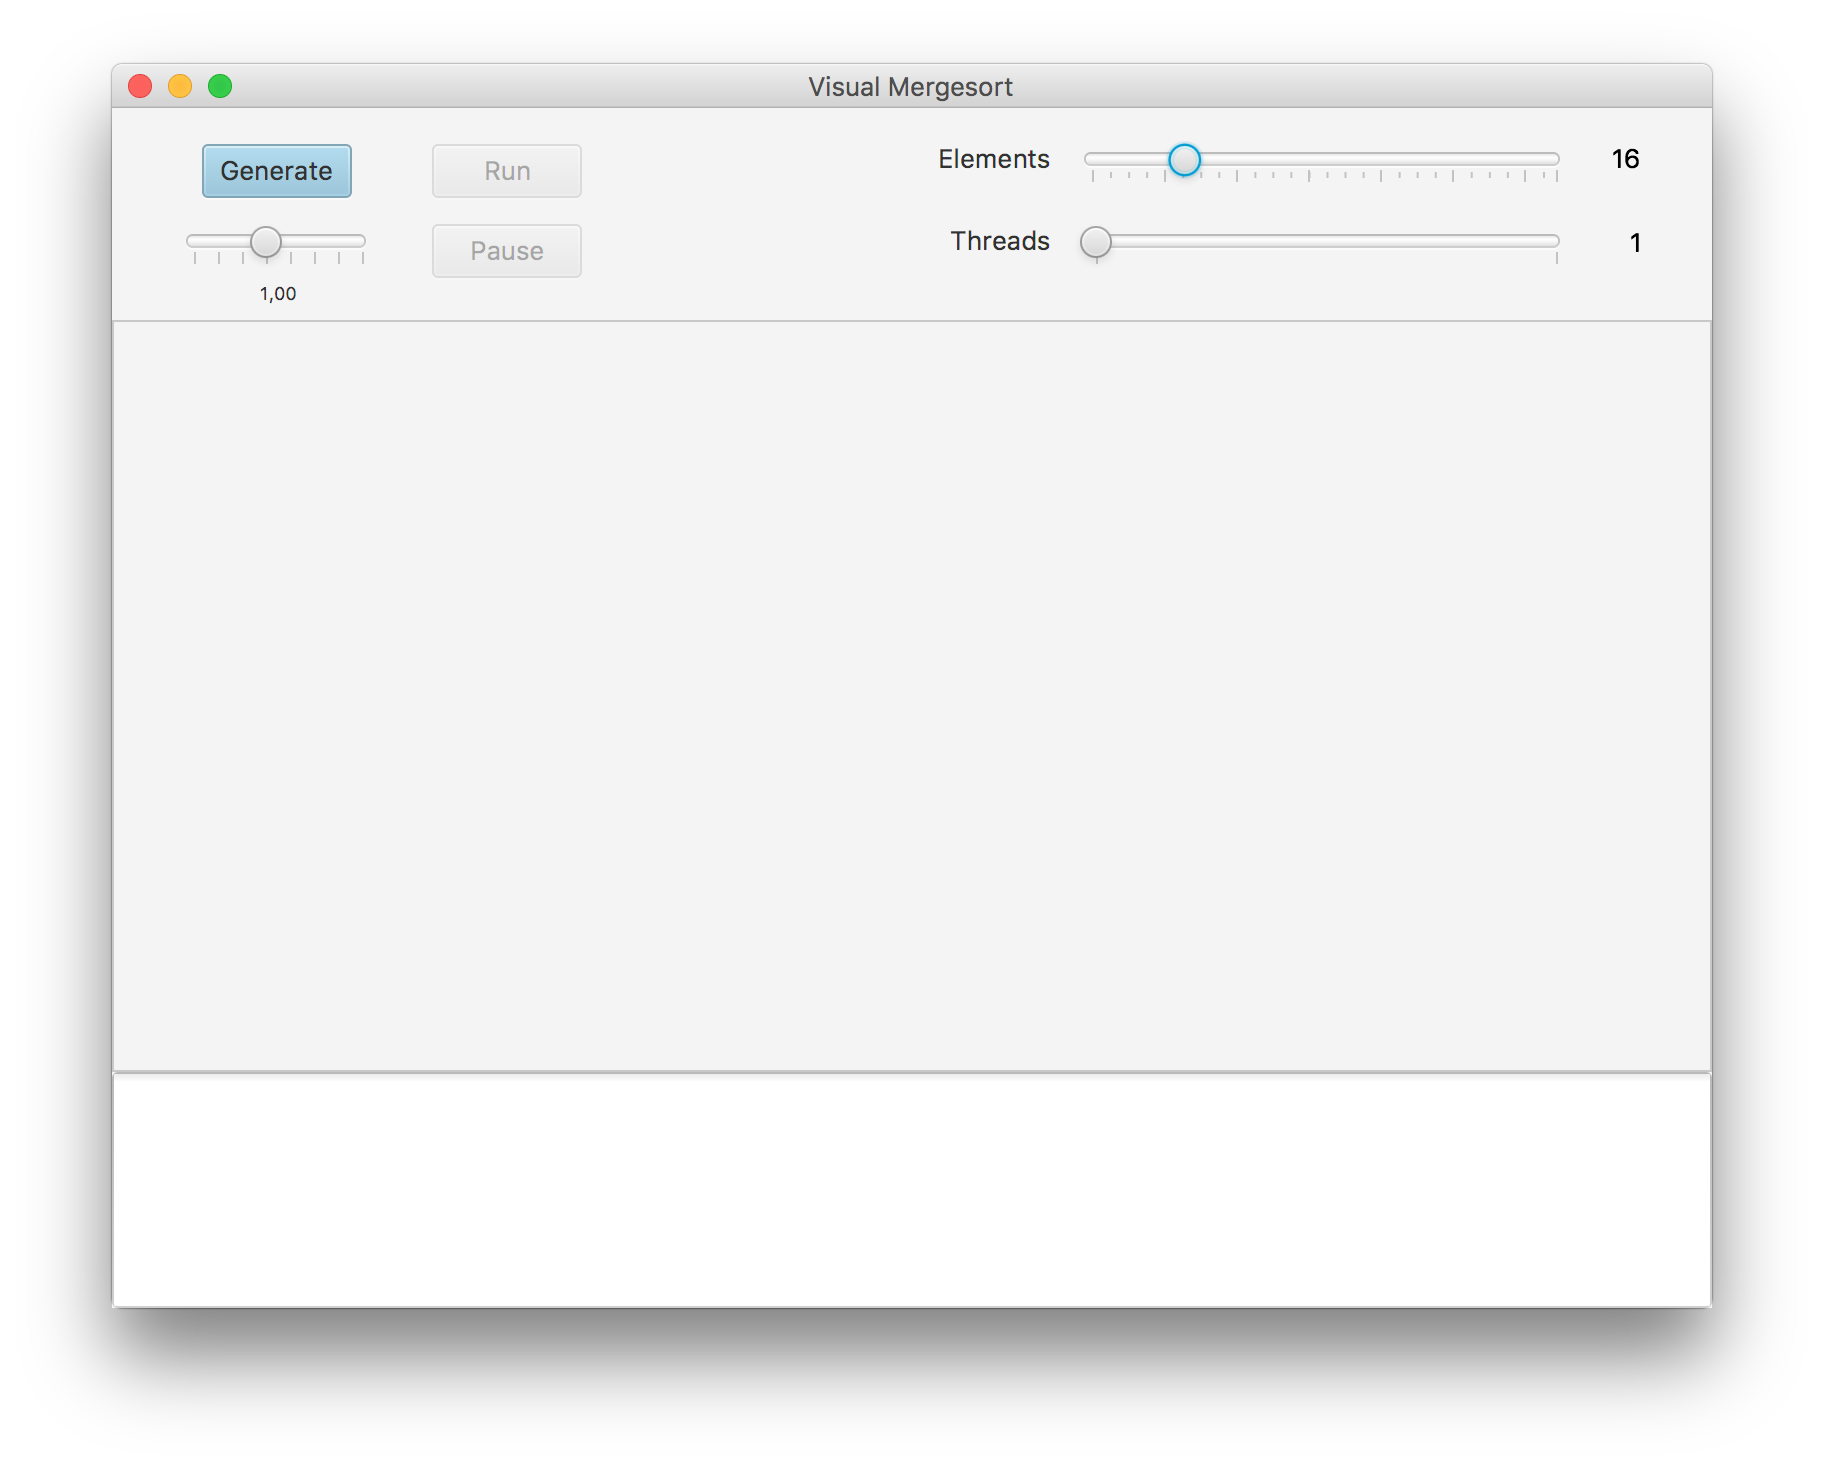
\includegraphics[width=0.75\linewidth]{bild1}
    \caption{Applikation direkt nach dem Starten}
    \label{figure:start-app}
\end{figure}

Über \texttt{ENTER} oder das Klicken auf \texttt{Generate} können direkt die über den Slider voreingestellten 16 Zufallselemente in willkürlicher Reihenfolge generiert werden. Alternativ kann über die Menüleiste \texttt{File} $\rightarrow$ \texttt{Generate Random Data} eine andere Reihenfolge ausgewählt werden. Um einen schnellen Start mit der gewünschten Menge zu ermöglichen, existieren folgende Shortcuts, welche optional verwendet werden können:

Je nach benutztem Shortcut wird eine andere Menge von Elementen auf der Zeichenfläche platziert. Der Slider für die Anzahl der zu zeichnenden Elemente gilt bei allen Optionen, außer bei der generierung von benutzerspezifischen Elementen (siehe unten).

\begin{description}
\item[STRG + B] Generiert eine Menge von Zufallszahlen in willkürlicher Reihenfolge (default). (Abbildung: \ref{figure:zufall})

\begin{figure}[!htb]
    \centering
      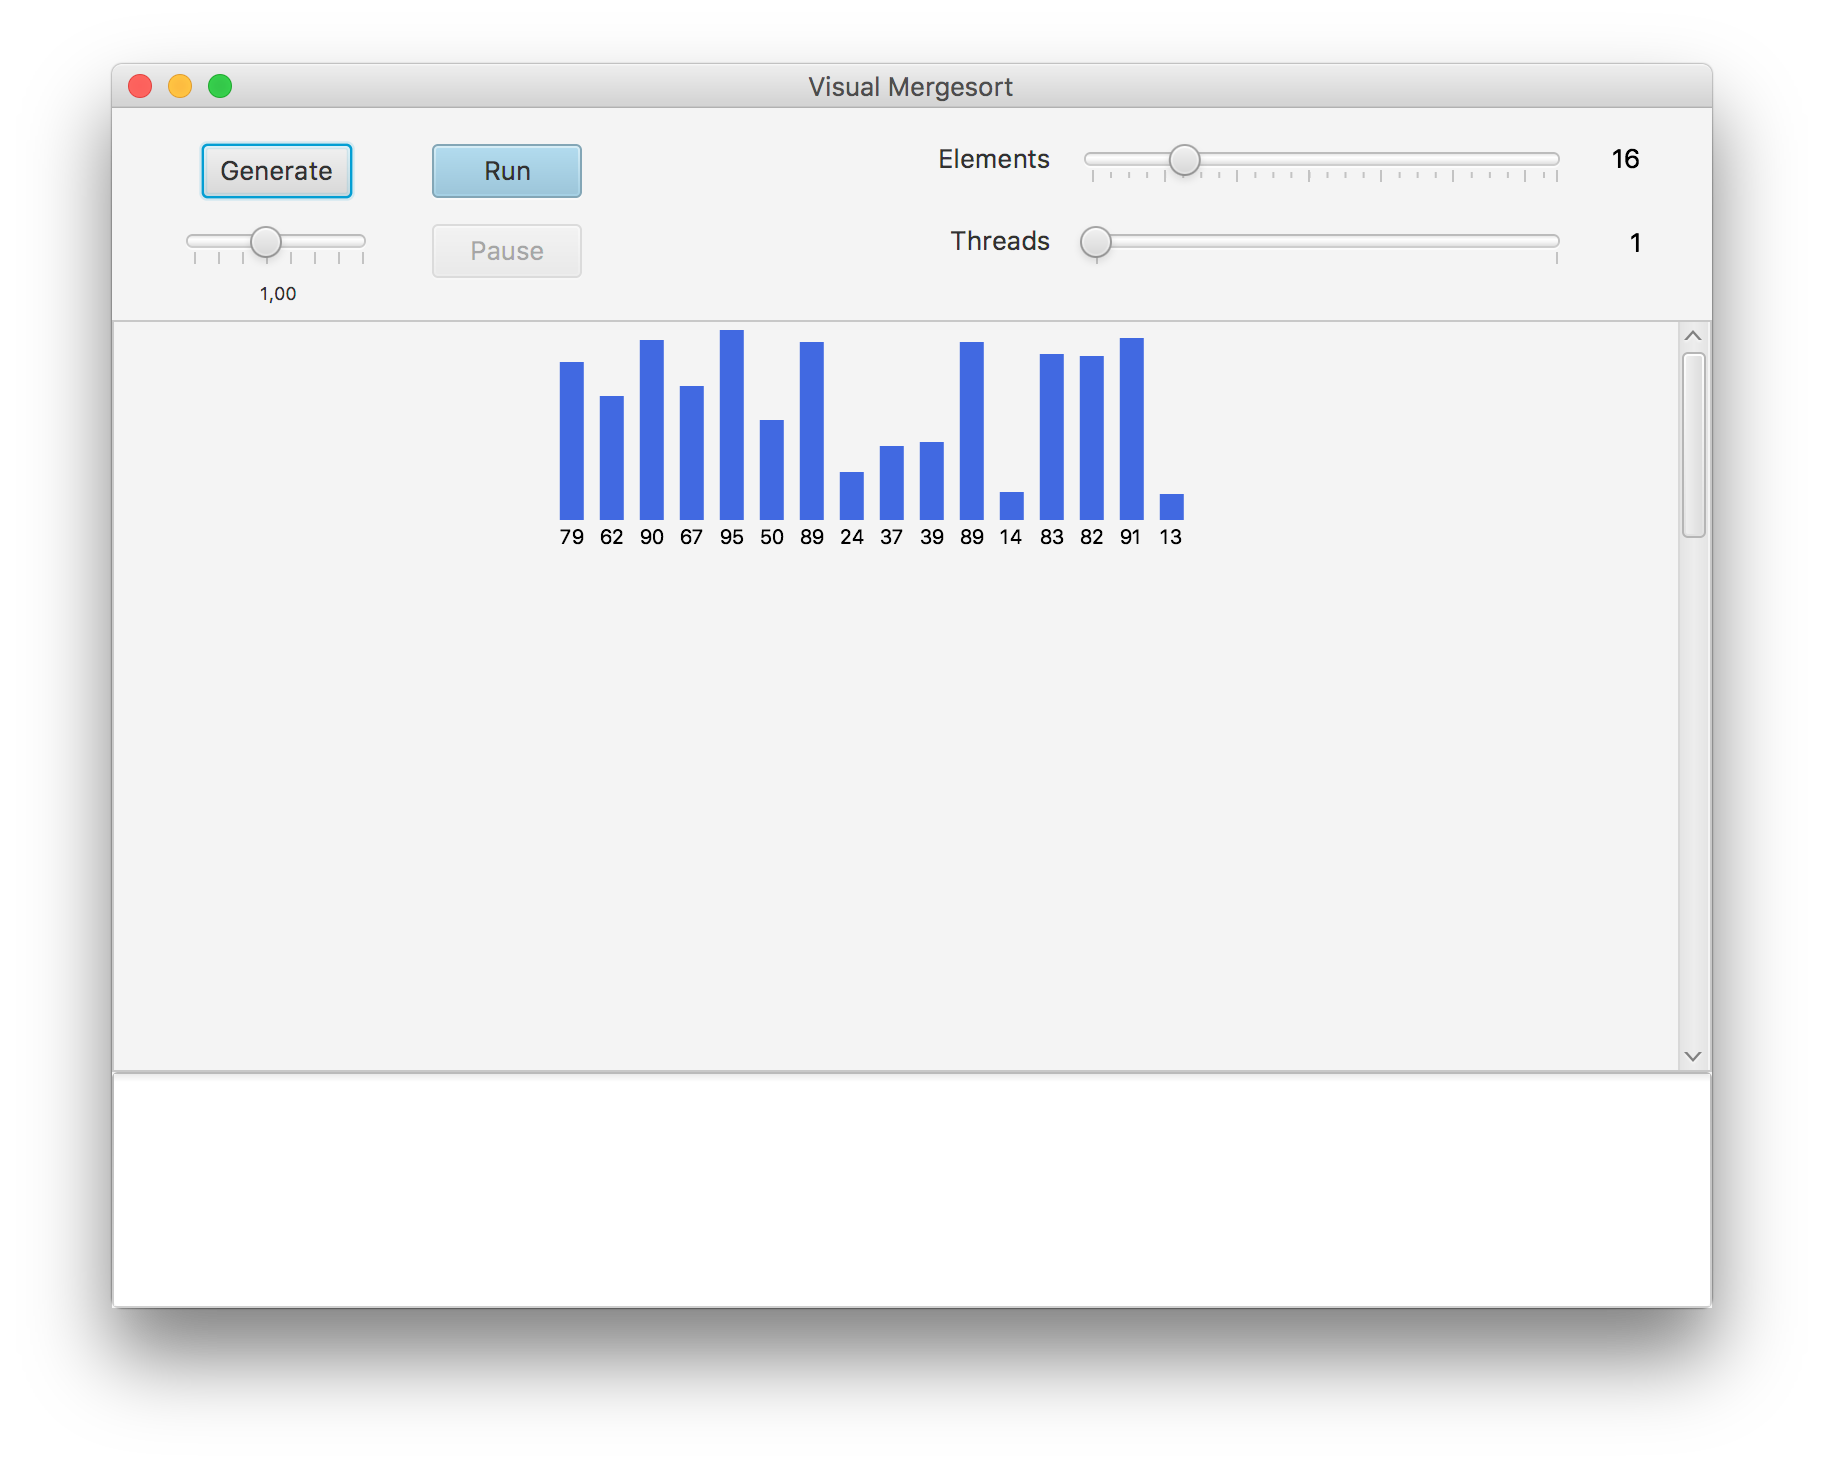
\includegraphics[width=0.75\linewidth]{bild2}
    \caption{Elemente in zufälliger Reihenfolge}
    \label{figure:zufall}
\end{figure}

\item[STRG + O] Generiert eine Menge von Zufallszahlen in vorsortierter, aufsteigender Reihenfolge. (Abbildung: \ref{figure:vorsortiert})

\begin{figure}[!htb]
    \centering
      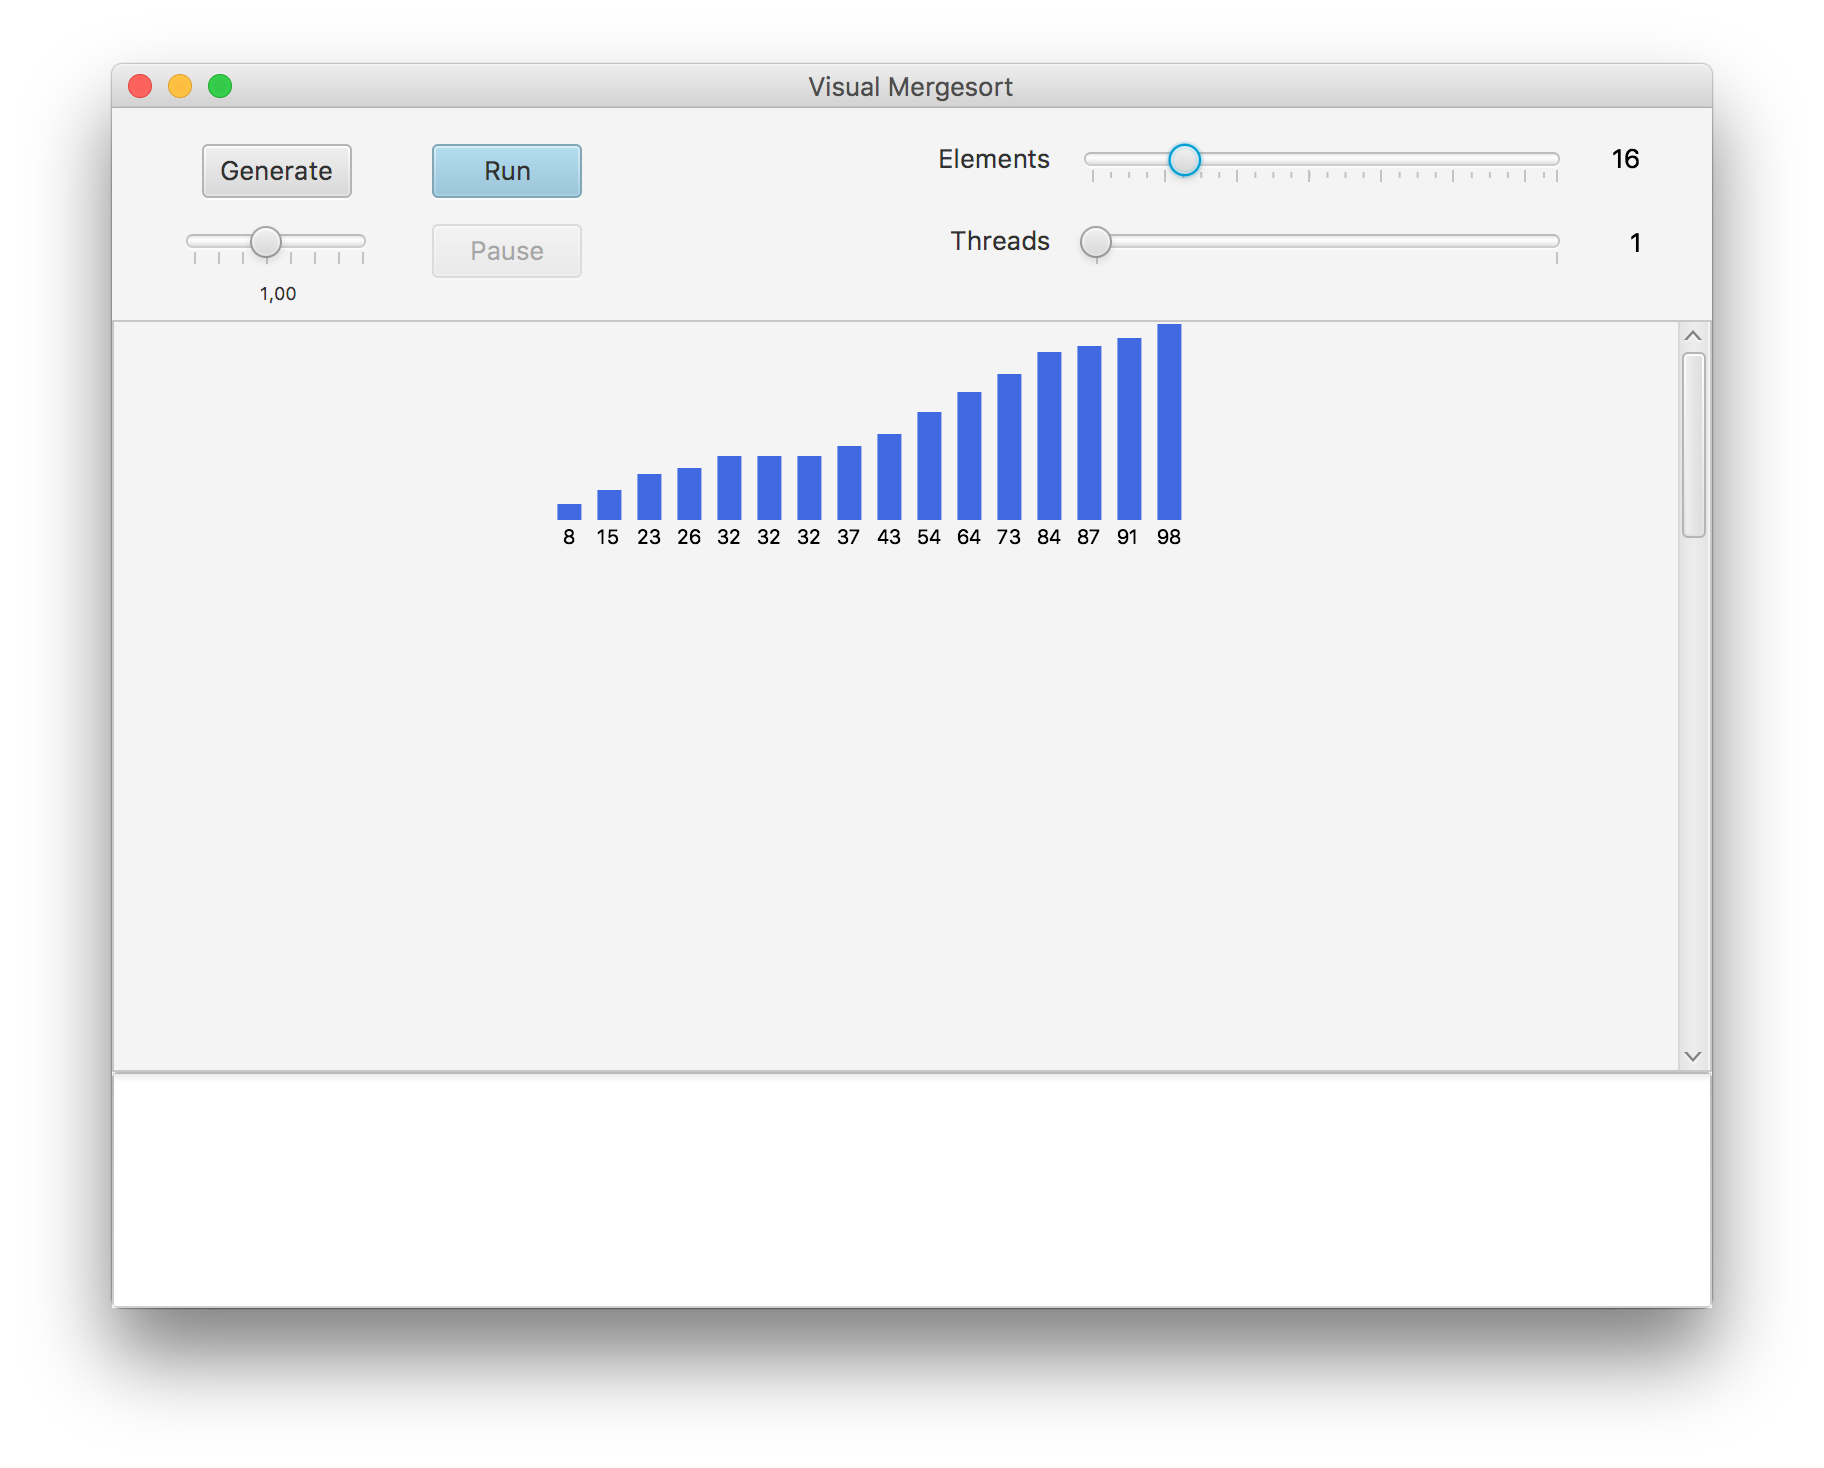
\includegraphics[width=0.75\linewidth]{bild6}
    \caption{Elemente vorsortiert in aufsteigender Reihenfolge}
    \label{figure:vorsortiert}
\end{figure}

\item[STRG + I] Generiert eine Menge von Zufallszahlen, welche absteigend sortiert ist. (Abbildung \ref{figure:inverse})

\begin{figure}[!htb]
    \centering
      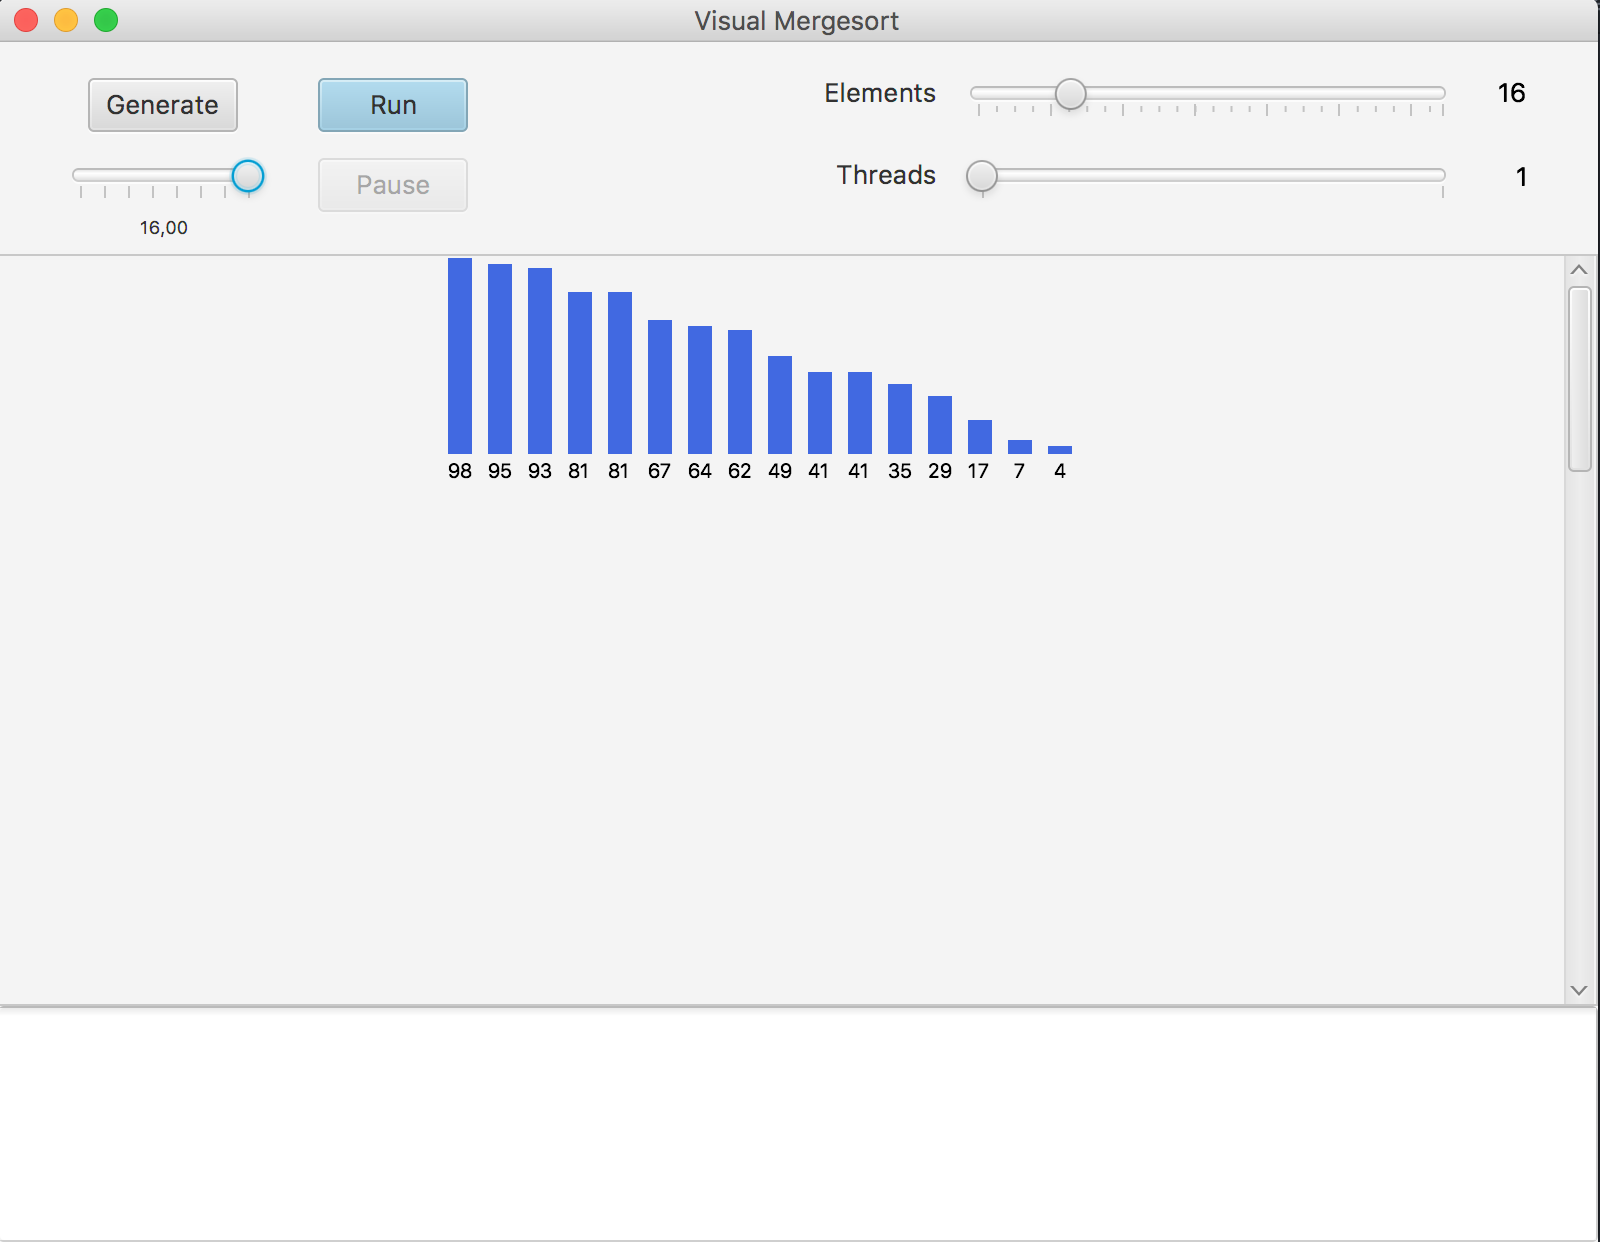
\includegraphics[width=0.75\linewidth]{bild7}
    \caption{Elemente vorsortiert in absteigender Reihenfolge}
    \label{figure:inverse}
\end{figure}

\item[STRG + U] Sowohl die Menge der Zahlen als auch die Reihenfolge kann über den Benutzer manuell eingegeben werden. Hierzu öffnet sich ein Fenster, bei dem die gewünschten Werte eingegeben werden. Dabei ist darauf zu achten, dass jeder Wert durch ein Komma vom nächsten Wert getrennt wird. (Abbildung \ref{figure:benutzer})

\begin{figure}[!htb]
    \centering
      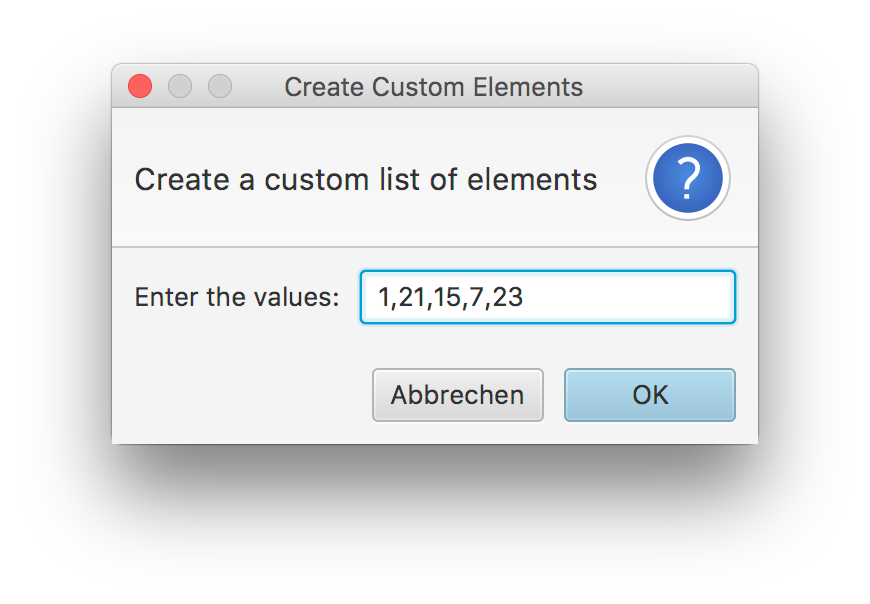
\includegraphics[width=0.75\linewidth]{bild8}
    \caption{Generieren von benutzerspezifischen Elementen}
    \label{figure:benutzer}
\end{figure}

Bestätigt man anschließend durch das Drücken auf den Button \texttt{OK}, erscheinen die eingegebenen Werte als Elemente auf der Zeichenfläche. (Abbildung \ref{figure:benutzer})

\begin{figure}[!htb]
    \centering
      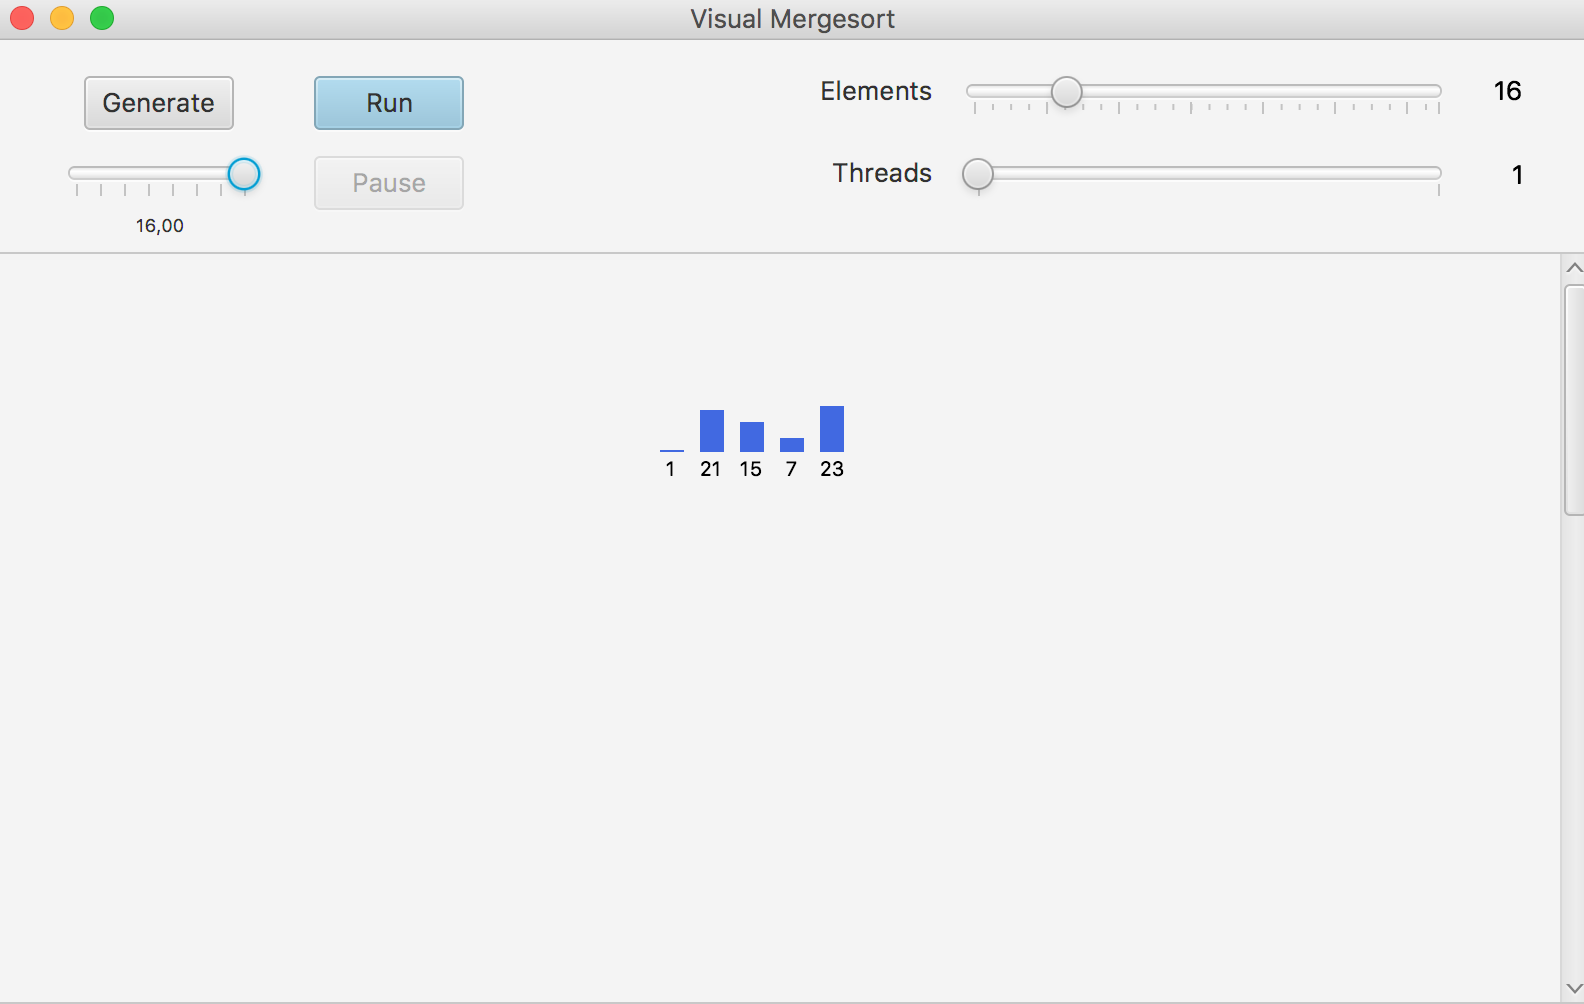
\includegraphics[width=0.75\linewidth]{bild9}
    \caption{Benutzerspezifische Elemente wurden generiert}
    \label{figure:benutzer2}
\end{figure}
\end{description}

Mit \texttt{ENTER}, einem Klick auf \textbf{Run} oder dem optionalen Shortcut \texttt{STRG + r} wird der Sortieralgorithmus gestartet. Über den Slider mit der Signatur \textit{Threads} kann die Anzahl der für den Algorithmus verwendeten Threads eingestellt werden. Hierbei kann man zwischen einem und zwei Threads wählen.\\
Wurde die Animation gestartet, kann diese jederzeit in ihrer Geschwindigkeit über den Regler unter dem Generate-Button variiert oder über den Button \textit{Pause} bzw. \textit{Play} komplett pausiert bzw. fortgesetzt werden. Beim Starten der Applikation fällt mit Sicherheit auf, dass sich das System automatisch zum Geschehen mitbewegt, um das Vorgehen besser zu visualisieren. Möchte man sich bestimmte Teile genauer ansehen, kann die Anwendung pausiert werden - Anschließend kann man sich frei auf der Zeichenfläche bewegen.

Darüber hinaus kann über den Menüpunkt View die Ansicht der Applikation zu jeder Zeit angepasst werden. Hier existieren die Optionen
\texttt{Toggle Log Console} und \texttt{Toggle Action Bar}. \texttt{Toggle Log Console} sorgt für das Ein- und Ausblenden der Konsole
im unteren Teil der Anwendung. Dadurch kann man bei Bedarf die zusätlichen Informationen zu \texttt{Split} und \texttt{Merge} ausblenden,
um mehr Platz für die eigentliche Animation zu schaffen. \texttt{Toggle Action Bar} ist hierbei aus den gleichen Gründen für das Ein- und Ausblenden
der Schalt- und Kontrollflächen im oberen Teil der Applikation zuständig. Zusätzlich können diese Funktionen optional auch über Tastenkombinationen ausgeführt
werden:

\begin{description}
\item[STRG + K] Blendet die Aktionsbar ein und aus.

\begin{figure}[!htb]
    \centering
      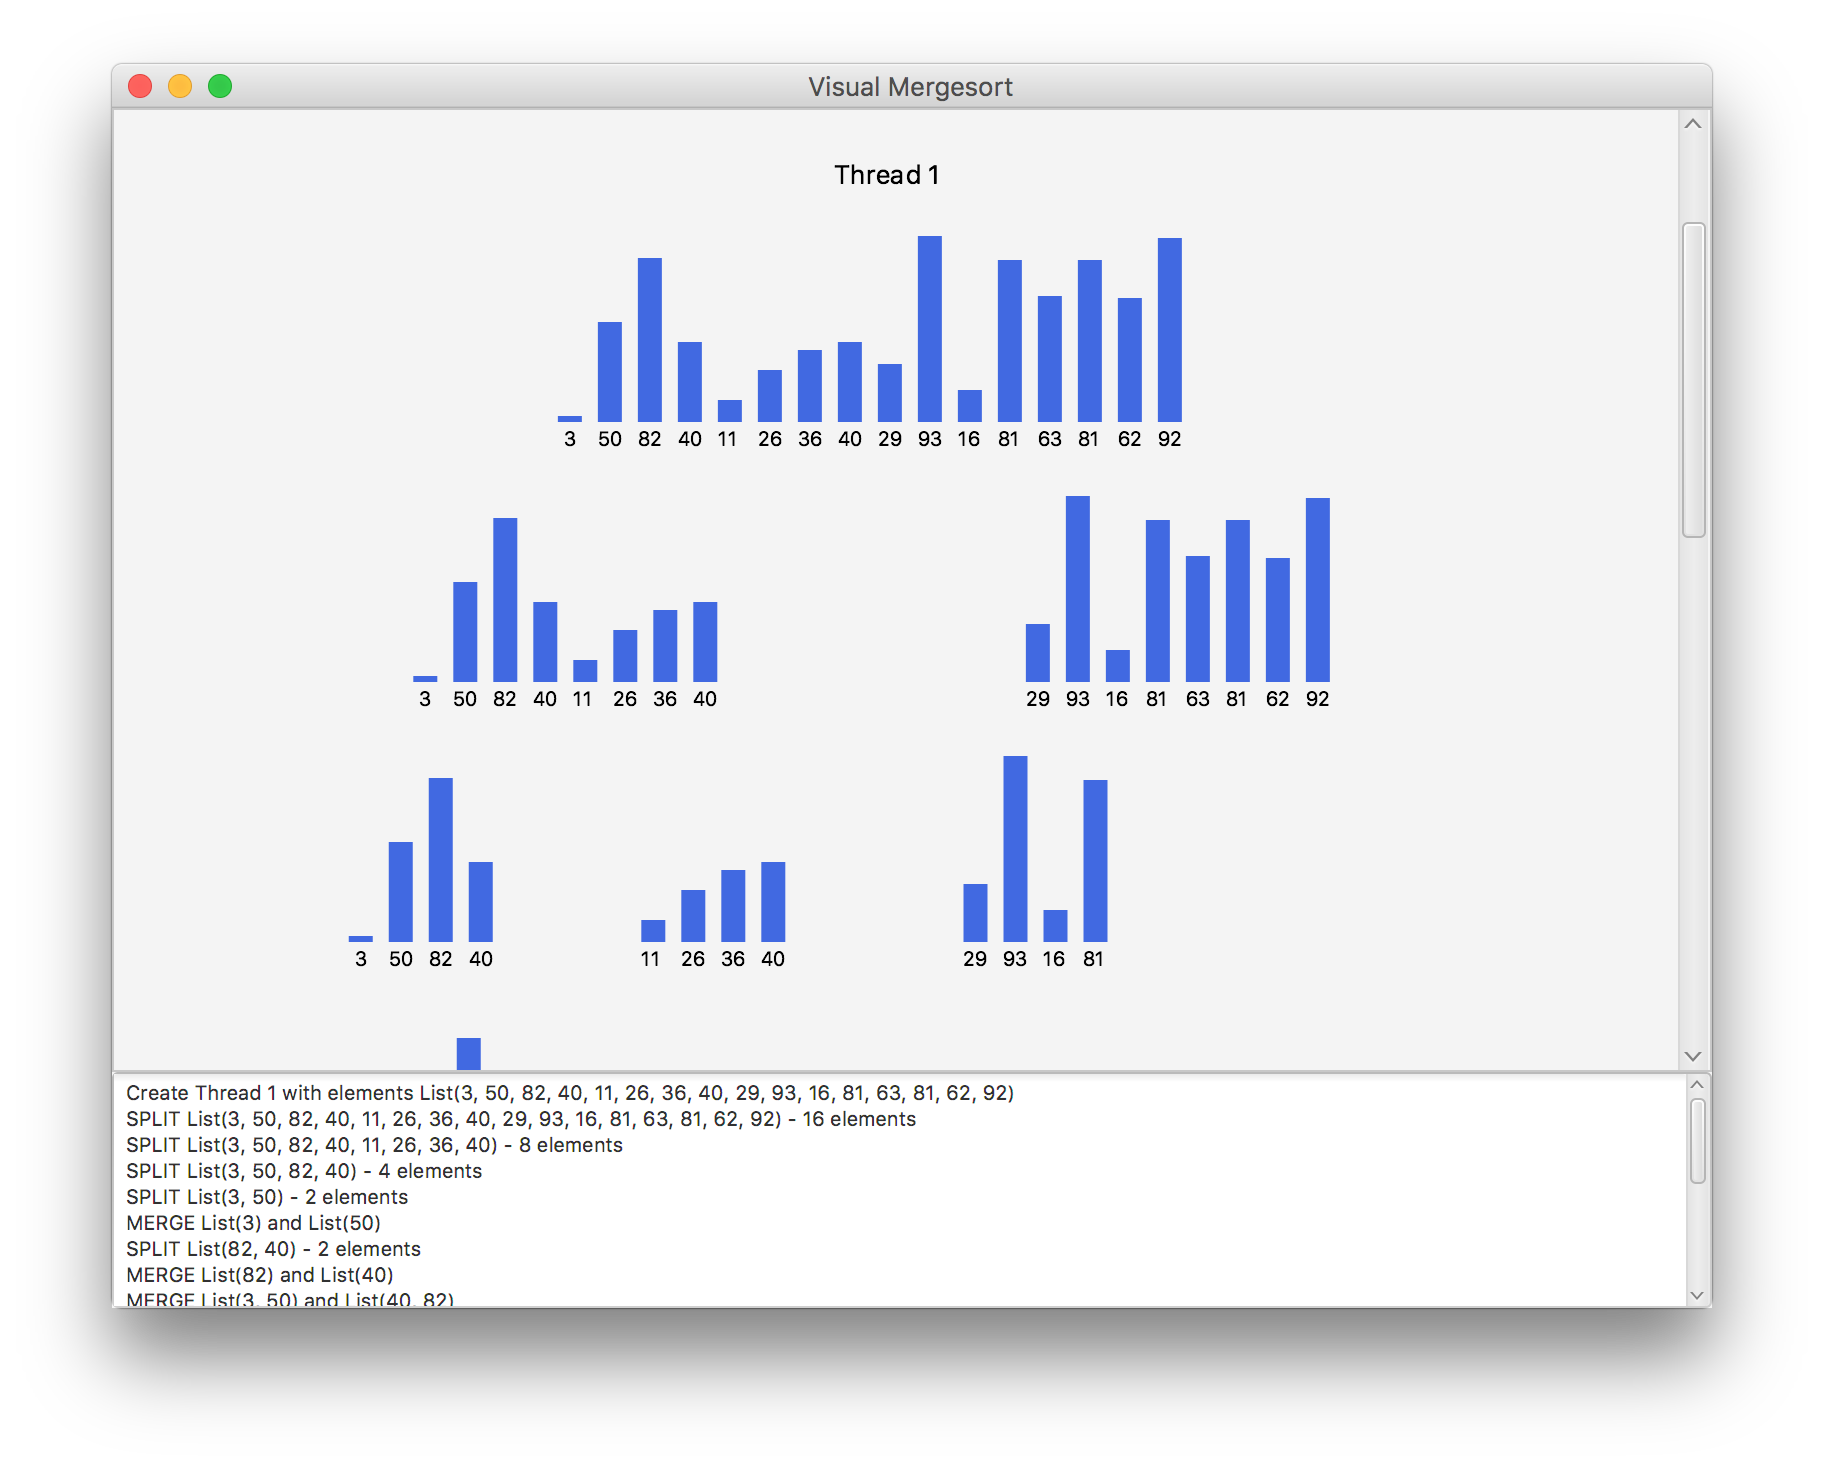
\includegraphics[width=0.85\linewidth]{bild10}
    \caption{Visual Mergesort mit ausgeblendeter Aktionsbar}
\end{figure}

\item[STRG + L] Blendet die Konsole ein und aus.

\begin{figure}[!htb]
    \centering
      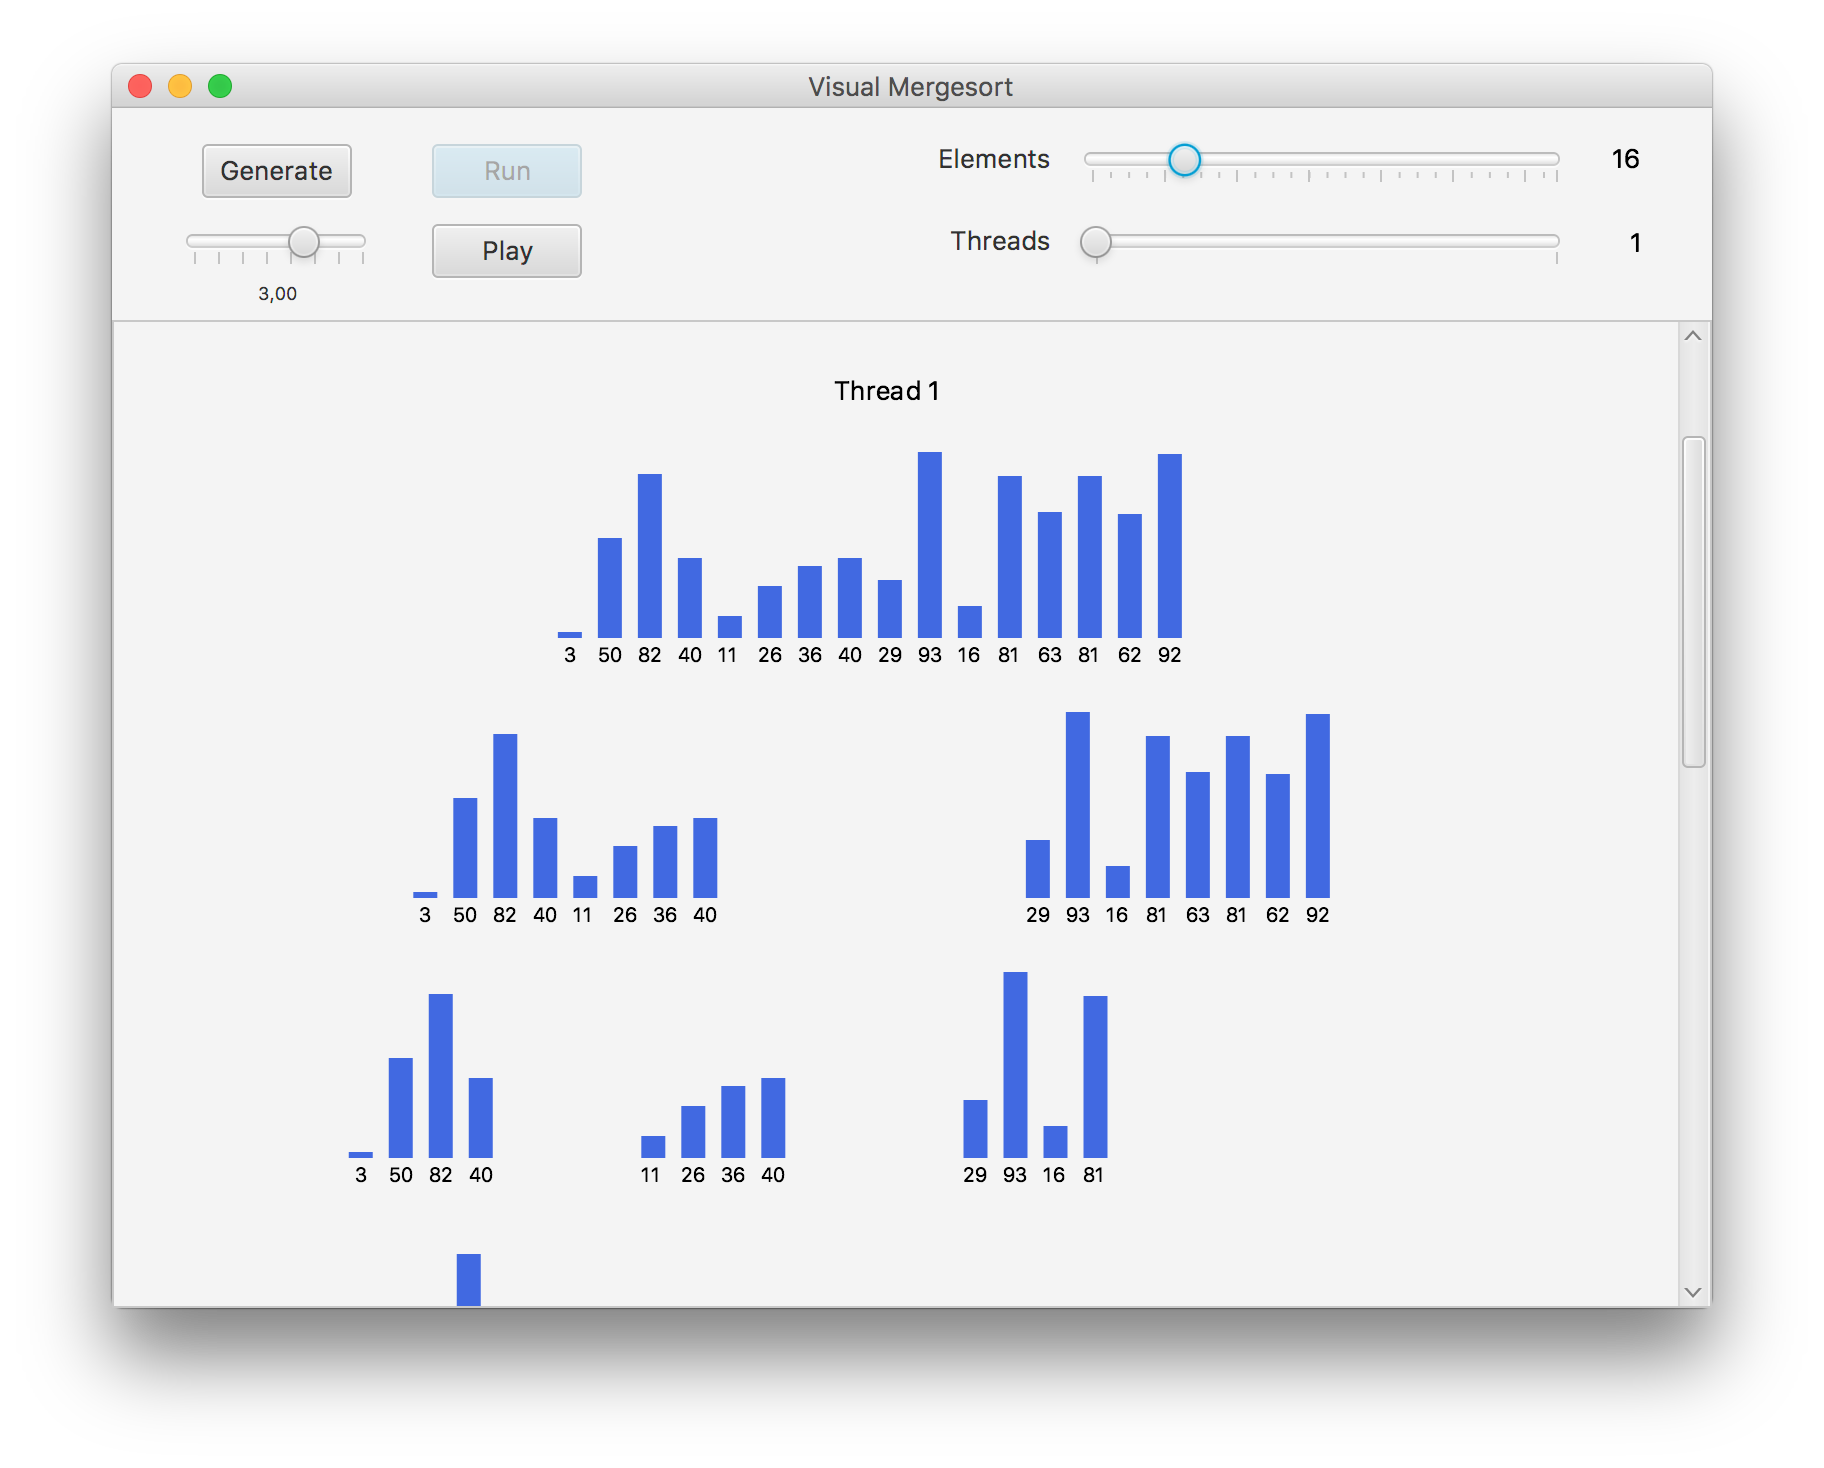
\includegraphics[width=0.75\linewidth]{bild11}
    \caption{Visual Mergesort mit ausgeblendeter Konsole}
\end{figure}
\end{description}

Um den Algorithmus effizienter zu machen, ist es möglich, beim Visual Mergesort die Anzahl der verwendeten Threads, die den Sortieralgorithmus ausführen, zu verändern. Dadurch kann sich der Benutzer vor Augen halten, wie der Mergesort parallelisiert werden kann, um dessen Leistung zu steigern. Wurde über den Slider \texttt{Threads} die Zahl 2 ausgewählt, wird die zu sortierende Liste beim Starten der Anwendung über \texttt{Run} direkt in zwei Listen geteilt, welche jeweils einem \texttt{Thread 1} und einem \texttt{Thread 2} zugewiesen werden:

\begin{figure}[!htb]
    \centering
      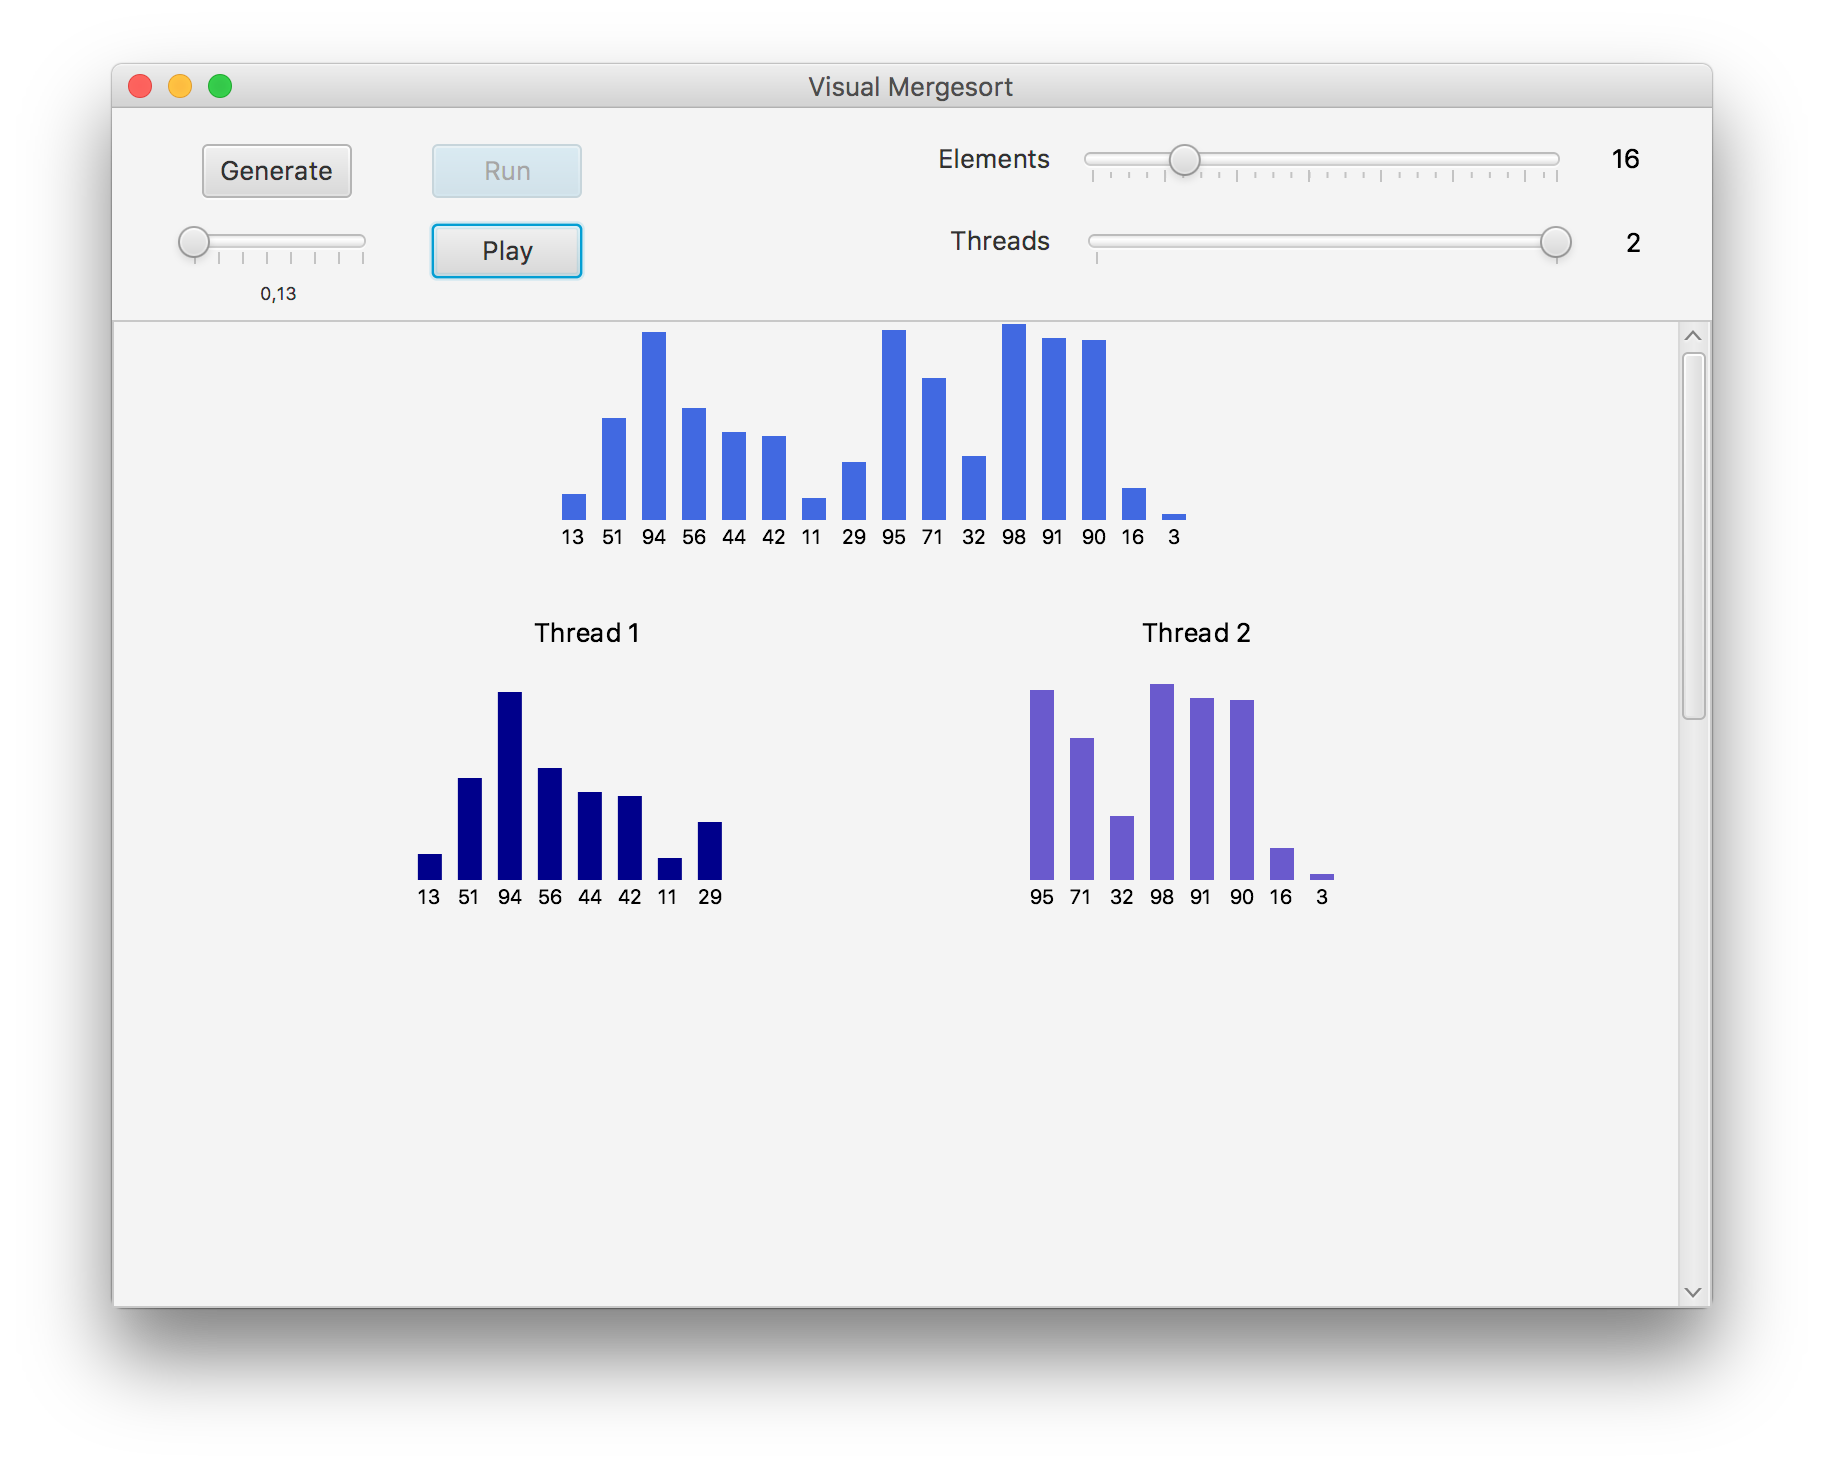
\includegraphics[width=0.75\linewidth]{bild12}
    \caption{Visual Mergesort mit zwei Threads}
\end{figure}

Ab hier führt jeder Thread den Mergesort-Algorithmus für die Liste durch, die ihm zugeteilt wurde, bis diese vollständig sortiert ist. Zum Schluss kommt es zu einem finalen Merge, bei dem die beiden durch die Threads generierten Teillisten zu einer Ganzen zusammengefügt werden. Hierbei kann es, beispielsweise bei einer ungeraden Anzahl an Ausgangselementen dazu kommen, dass ein Thread mehr Zeit benötigt, als der andere, da dieser ein Element weniger sortieren muss. Für diesen Sonderfall wird die Autoscrollfunktion automatisch deaktiviert, da die Threads an verschiedenen Stellen auf der Zeichenfläche arbeiten. Vor dem final Merge wartet der eine Thread auf den anderen, bis dessen Liste auch sortiert ist.

\begin{figure}[!htb]
    \centering
      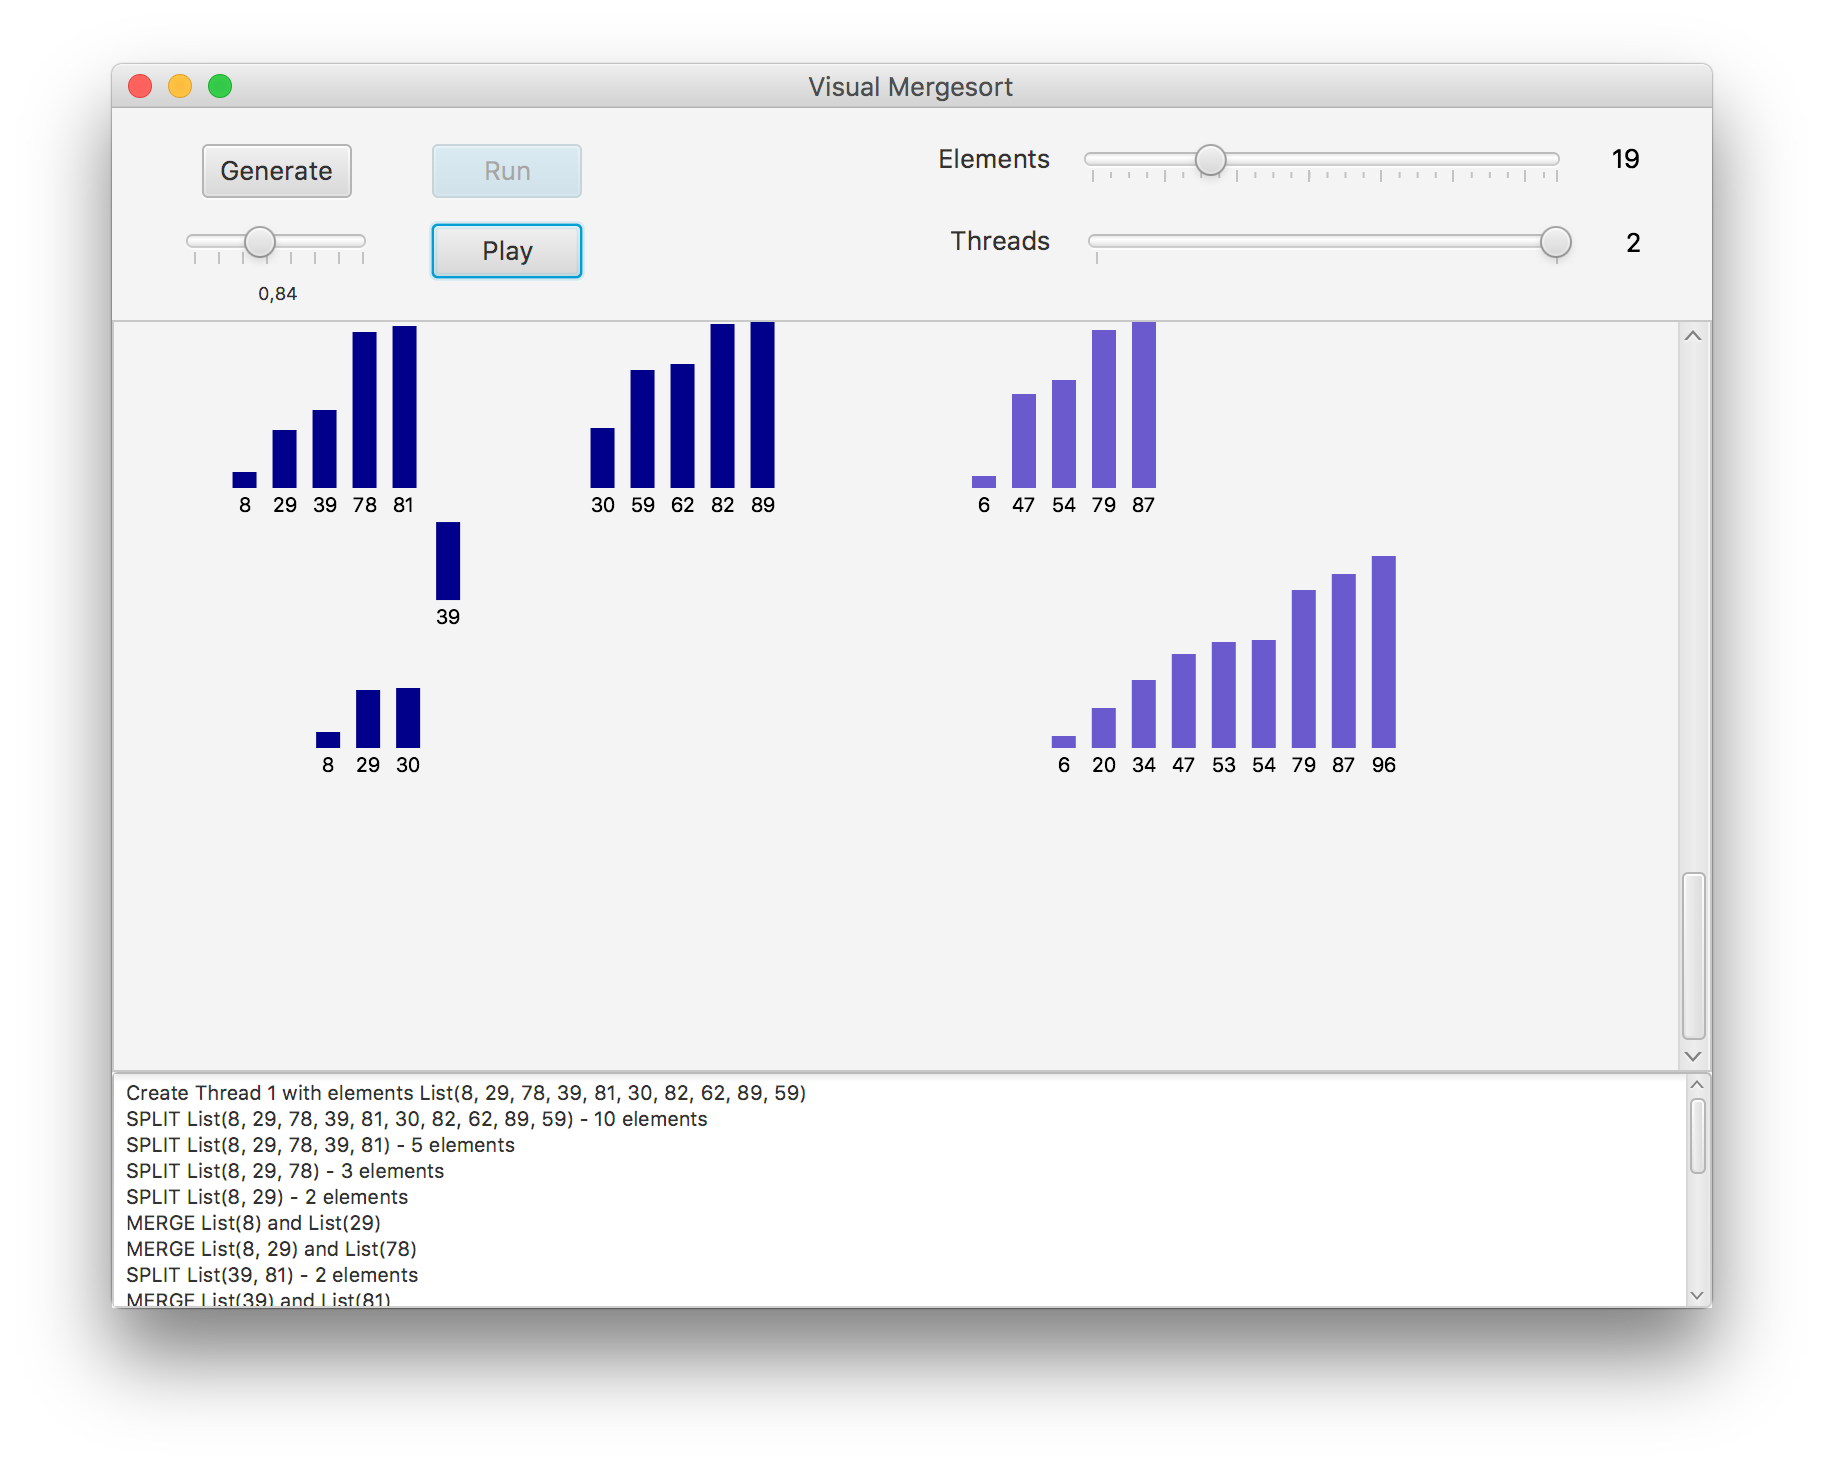
\includegraphics[width=0.75\linewidth]{bild13}
    \caption{Thread 2 wartet auf Thread 1}
\end{figure}
